\documentclass{article}

\usepackage{graphicx}
\usepackage[utf8]{inputenc}
\usepackage[T1]{fontenc}
\usepackage[francais]{babel}
\usepackage{hyperref}
\usepackage{amsmath,amsfonts,amssymb}
\usepackage{Tkz-Tab}
\usepackage{wrapfig}
\usepackage{verbatim}
\usepackage{array}

\begin{document}

\title{Gestion de flux dans le réseau
	\smallbreak
	TD n\degre5
	\smallbreak
	Modélisation mathématique
	\smallbreak
	Q4}
\author{Sibylle Roux \and Juliette Arazo \and Nicolas Le Gallo \and Tanguy Thomas}

\maketitle

\newpage

\tableofcontents

\newpage

\section{Essaies randoms}

\subsection{}

\section{Etude mathématique de la loi tente}

\subsection{Densité}

\subsubsection{Fonction}

$$
f(x)=\left\{
	\begin{array}{ll}
		1-|x| & \mbox{si} -1<=x<=1\\
		0 & \mbox{sinon}
	\end{array}
\right.
$$

\subsubsection{Représentation graphique}
\begin{center}
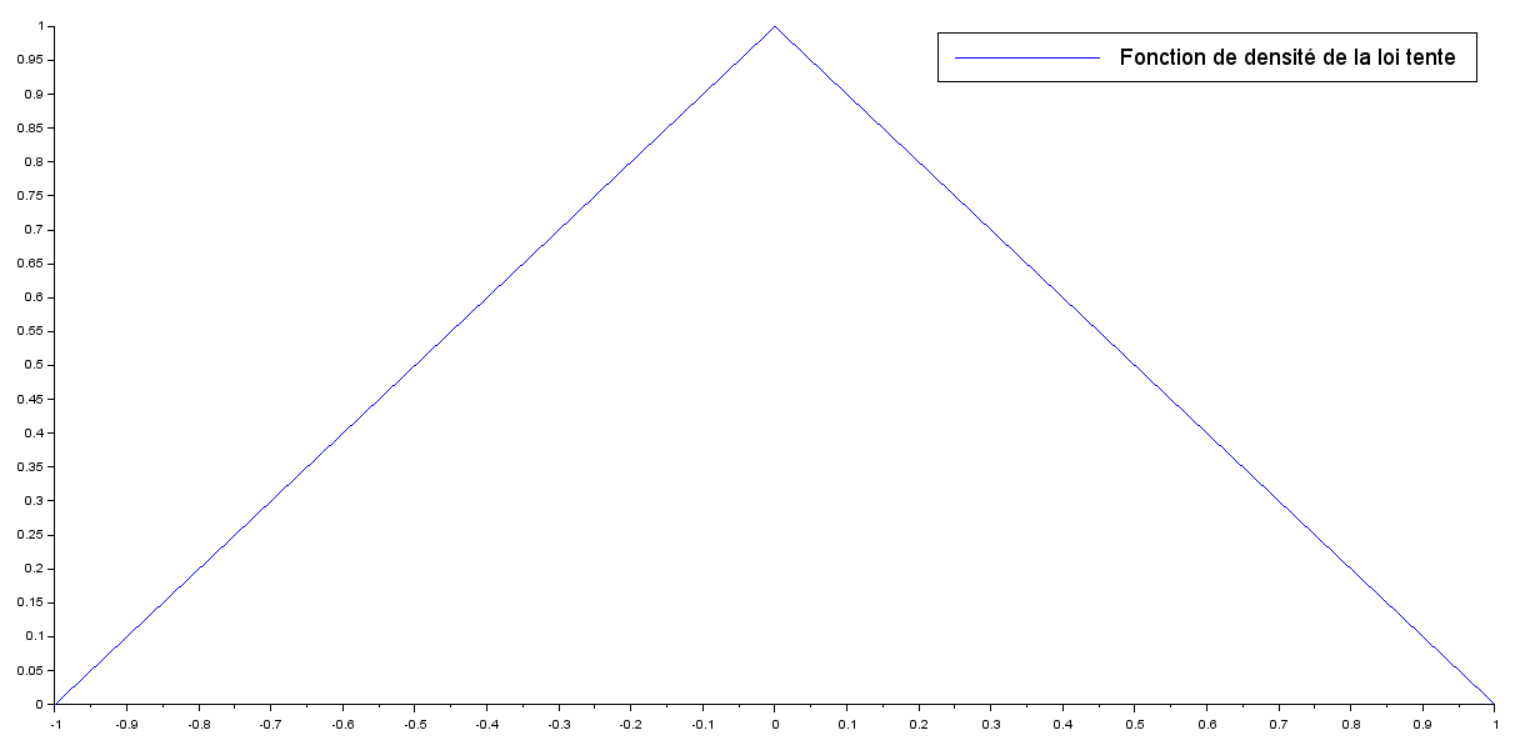
\includegraphics[width=425px]{img/tente.png}
\end{center}
\paragraph{}

\newpage

\subsection{Fonction de répartition}

\subsubsection{Fonction}

\begin{align}
f(x)=\left\{
	\begin{array}{llll}
		f(x)=0 &\mbox{pour } x<-1\\
		f(x)=1+x & \mbox{pour } -1<x<0 \\
		f(x)=1-x & \mbox{pour } 0<x<1 \\
		f(x)=0 & \mbox{pour } x>1 \\
	\end{array}
\right. 
\end{align}
\begin{align}
<=>
F(x)=\left\{
	\begin{array}{llll}
		\displaystyle \int_{- \infty }^{x} 0 \, \mathrm{d}x &\mbox{pour } x<-1\\
		\displaystyle \int_{- \infty }^{-1} 0 \, \mathrm{d}x+\displaystyle \int_{-1 }^{x} 1+x \, \mathrm{d}x &\mbox{pour } -1<x<0\\
		\displaystyle \int_{- \infty }^{-1} 0 \, \mathrm{d}x+\displaystyle \int_{-1 }^{0} 1+x \, \mathrm{d}x + \displaystyle \int_{0}^{x} 1-x \, \mathrm{d}x &\mbox{pour } 0<x<1\\
		\displaystyle \int_{- \infty }^{-1} 0 \, \mathrm{d}x+\displaystyle \int_{-1 }^{0} 1+x \, \mathrm{d}x + \displaystyle \int_{0}^{1} 1-x \, \mathrm{d}x+\displaystyle \int_{1}^{x} 0 \, \mathrm{d}x &\mbox{pour } x>1\\
	\end{array}
\right. 
\end{align}
\begin{align}
<=>
F(x)=\left\{
	\begin{array}{llll}
		0 &\mbox{pour } x<-1\\
		0 + \displaystyle \int_{-1 }^{x} 1+x \, \mathrm{d}x &\mbox{pour } -1<x<0\\
		0+\frac{1}{2}+\displaystyle \int_{0}^{x} 1-x \, \mathrm{d}x &\mbox{pour } 0<x<1\\
		0+\frac{1}{2}+\frac{1}{2}+\displaystyle \int_{1}^{x} 0 \, \mathrm{d}x &\mbox{pour } x>1\\
	\end{array}
\right. 
\end{align}
\begin{align}
<=>
F(x)=\left\{
	\begin{array}{llll}
		0 &\mbox{pour } x<-1\\
		\displaystyle \int_{-1 }^{x} 1+x \, \mathrm{d}x &\mbox{pour } -1<x<0\\
		\frac{1}{2}+\displaystyle \int_{0}^{x} 1-x \, \mathrm{d}x &\mbox{pour } 0<x<1\\
		1 &\mbox{pour } x>1\\
	\end{array}
\right. 
\end{align}
\begin{align}
<=>
F(x)=\left\{
	\begin{array}{llll}
		0 & \mbox{pour } x<-1\\
		\frac{1}{2} + x + \frac{x^2}{2}\\
		\frac{1}{2} + x - \frac{x^2}{2}\\
		1 & \mbox{pour } x>1\\
	\end{array}
\right.
\end{align}



\subsubsection{Représentation graphique}
\begin{center}
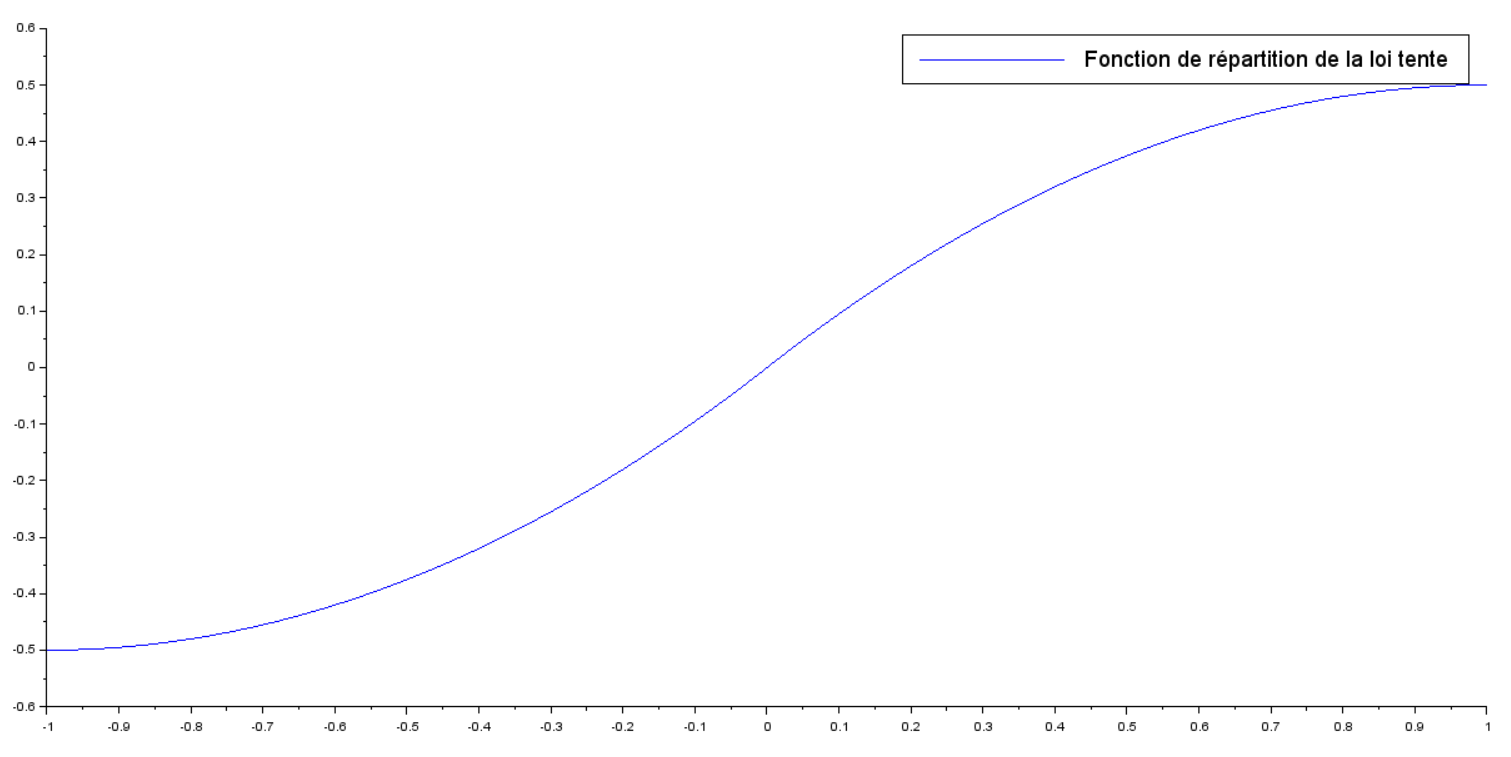
\includegraphics[width=425px]{img/tente_repartition.png} %TODO FAUX A CHANGER
\end{center}
\paragraph{}

\subsection{Inverse}

\part{Conclusion}
\paragraph{}

\newpage
\appendix

\section{}

\subsection{}

\subsubsection{}
\begin{verbatim}
\end{verbatim}

%----------------------------------


\end{document}